 \documentclass{article} %A4
\usepackage[a4paper,left=1.9cm, right=2.1cm,top = 1.2cm,bottom=2.3cm]{geometry}
\usepackage[utf8]{inputenc}%Umlaute
\usepackage[ngerman]{babel} %Texttrennung
\usepackage{graphicx}	%Grafiken
\usepackage{amssymb}
\usepackage{amsmath}
\usepackage{url}
\usepackage{listings}
\usepackage{color}
\usepackage{hyperref}
\usepackage{framed}
\usepackage{algpseudocode}
\usepackage{tikz}
\usepackage{enumitem}
\usepackage{multicol}
\usepackage[xindy,nonumberlist]{glossaries}
\makeglossaries
\usepackage[labelformat=empty]{caption}
\title{Zusammenfassung - Advanced Communications}
\author{
	Marc Meier, CD
}




\begin{document}
\maketitle
\begin{framed}Korrektheit und Vollständigkeit der Informationen sind nicht gewährleistet.
Macht euch eigene Notizen oder ergänzt/korrigiert meine Ausführungen!
\end{framed}
\setcounter{tocdepth}{1}
\tableofcontents
\newpage

\section{Grundlagen}

% 010, 020
\subsection{Grundprinzipien und Entwicklung des Internets}
Das Internet entwickelte sich ab den 1960er Jahren.
Es ging aus dem am Ende des Jahrzehnts entstandenen, vornehmlich militärisch und akademisch geprägten ARPA-Net hervor.
Heutzutage wird es international kommerziell, industriell und auch akademisch (Katzenbilder) genutzt.
Bei seiner Entstehung war vor allem eine dezentrale Struktur ohne zentrale Verwaltung von Interesse.
Grund hierfür war die Angst des amerikanischen Department of Defense, dass eine atomarer Angriff zentrale Kommunikationspunkte außer Kraft setzen könnte.
Die Kommunikation findet über hochgradig vernetzte Knoten mithilfe von Paketen statt.

Literatur: \cite{abbate2000inventing, baran1964distributed}
\subsection{Packet Switching}
Paketvermittelte Übertragung bedeutet die Abkehr von der leitungsbasierten Vermittlung.
Dabei werden längere Nachrichten in Datenpakete aufgeteilt und voneinander unabhängig versendet.
Dies ermöglicht eine faire Verteilung der Leistungskapazität und redundante Wege bei einem Ausfall von Knoten oder Verbindungen.
Im Gegenzug können konstante Bandbreiten nicht ohne Weiteres (Abschnitt \ref{sec:qos}) gewährleistet werden, ebenso ergeben sich unterschiedliche Laufzeiten von Paketen.

\subsection{Dezentrale Verwaltung des Internets}

\subsubsection{Prinzipien}

\begin{itemize}
\item Keine zentrale Verwaltung oder Behörde (trotz Einflussnahme)
\item Demokratisches Zusammenwirken der Beteiligten / Wahlen
\item Selbstorganisation
\item Standards dort, wo sie erforderlich sind
\item Dynamisch, offen für Neuigkeiten	
\end{itemize}

\subsubsection{Organisationen}

\begin{description}
\item[ICANN:] Vergibt IP-Adressen und betreibt die DNS-Rootserver.
\item[IETF:] Standardisierung von Protokollen in RFCs \cite{rfc3233}
\item[RIPE:] Administration und technische Koordination
\item[RIPE NCC:] Adressvergabe in Europa und Zentralasien, Verwaltung der WHOIS-Datenbank.
\item[DENIC eG:] Domain-Verwaltung für die Zone .de
\end{description}

\subsection{Standards}
Standards ermöglichen die Kooperation im Netzwerk, nur durch sie können Geräte verschiedener Hersteller miteinander kommunizieren.
Sie können textuell, mithilfe einer Referenzimplementierung oder anhand von Automaten (meist für zustandsbehaftete Protokolle) festgelegt werden.\\
Sie müssen verschiedenen Ansprüchen genügen: Vollständig, eindeutig (widerspruchsfrei) und stabil 

\begin{description}
\item[Protokoll] Standardisierte Regeln (Vorschriften) und Vereinbarungen zu
Form, Ablauf, Steuerung und Sicherung (Fehler) der
Datenübertragung in und zwischen Rechnernetzen, zwischen
Einzel-Rechnern und zwischen Rechnern und
Peripheriegeräten.
\item[Standard] Ein Standard wird von den verschiedensten internationalen und
nationalen Organisationen sowie von großen Firmen erstellt.
Ein Standard wird als verbindliche oder unverbindliche
(empfohlene) Festlegungen schriftlich niedergelegt.
\end{description}

Ablauf einer Standardisierung bei RFCs:
\begin{enumerate}
	\item \textbf{Proposed Standard}: Vollständige, konsistente Spezifikation vorhanden
	\item \textbf{Draft Standard}: Mindestens 2 unabhängige, interoperable Implementierungen
	\item \textbf{Standard}: Operationell stabil
\end{enumerate}
\textbf{Weitere Status:} \emph{Experimental}, \emph{Informational} und \emph{Historic}.
\subsection{Netze, Autonome Systeme und Schichten}
Große Teile des Internet-Backbones werden von wenigen Firmen bereitgestellt (Tier-1).
Diese werden an einigen Knotenpunkten verbunden.
Wichtiger Knotenpunkt in Deutschland ist DE-CIX in Frankfurt/Main.
Man unterteilt folgende \textbf{Netzwerk-Schichten}:
\begin{description}
	\item[Tier 1]: Ein Netzwerk, das mit allen anderen Tier-1-Netzwerken verbunden ist; \emph{Internet-Backbone}; z.B. ATDN, GX, AT\&T...
	\item[Tier 2]: Netzwerk, das mit vielen Netzwerken verbunden ist, aber Transit \emph{einkauft}, um einige Bereiche des Internets zu erreichen; z.B. Deutsche Telekom
	\item[Tier 3]: Ein Netzwerk, das ausschließlich Transit \emph{einkauft}, um das
	Internet zu erreichen
\end{description}
\textbf{Autonome Systeme} sind Ansammlungen von IP-Netzen, die als Einheit verwaltet werden.
Innerhalb kommt ein einheitliches Routing-Protokoll zum Einsatz.
Autonome Systeme sind untereinander verbunden und
bilden das Internet.

\subsection{Begriffe}
%TODO
\begin{description}
	\item[Datendurchsatz] Bla
	\item[Datenrate] Bla
	\item[Routing] Bla
\end{description}

\section{Protokolle}
Protokolle können als Vorschrift betrachtet werden, wie sich verhalten werden soll. Zur Interaktion wird beschrieben, welches Datenformat und wann etwas geschickt werden darf.
\subsection{Zustandslose und zustandsbehaftete Protokolle}
Bei \textbf{zustandslosen Protokollen} wird jede Anfrage in einer eigenständigen Transaktion ausgeführt, es existieren keine Vorbedingungen oder Sitzungsinformationen (UDP, HTTP, TFTP).
\textbf{Zustandsbehaftete Protokolle} hingegen merken sich den aktuellen Zustand mithilfe einer Sitzung.
Nachfolgende Anfragen können auf die Sitzungsinformationen zugreifen.
Diese Zustandsübergänge können durch endliche Automaten dargestellt werden.
Beispiele sind FTP, TCP und SMTP.

\subsection{OSI-7-Schichten-Modell}

\begin{enumerate}
	\item Physical Layer / Bitübertragung
	\item Data Link Layer / Sicherungsschicht / Datenübertragungsschicht
	\item Network Layer / Vermittlungsschicht
	\item Transport Layer
	\item Session Layer / Sitzungsschicht
	\item Presentation Layer / Darstellungsschicht
	\item Application Layer / Anwendungsschicht
\end{enumerate}

Gute \textbf{Eselsbrücken} sind:
\begin{itemize}
	\item Alle deutschen Studenten trinken verschiedene Sorten Bier (deutsche Bezeichnungen, 7-1)
	\item An dem Samstag trug Verena 'nen String in Blau (deutsche Bezeichnungen, 7-1)
	\item Alle poppen Susis Tante nach der Party (deutsche Bezeichnungen, 7-1)
	\item Physiker, die nicht trinken sind potentielle Attentäter (deutsche/englische Bezeichnungen, 1-7)
	\item Alibaba präsentiert sich täglich nackt dem Personal
	\item  Please Do Not Throw Salami Pizza Away (englisch, 1-7)
\end{itemize}

Jede Schicht $n$ nutzt die darunterliegende Schicht $n-1$ um mit dem Kommunikationspartner zu kommunizieren.
Daten höherer Schichten werden in niederen Schichten umkapselt.
Die Bezeichnung der Pakete ist je nach Schicht unterschiedlich:
\begin{description}
	\item[Data Link Layer]: (Ethernet-)Frame
	\item[Network Layer]: Paket
	\item[Transport Layer]: Fragment
\end{description}

\subsection{Ethernet}
\label{subsec:ethernet}
Das Ethernet-Protokoll wirkt auf den Layern 1 + 2 und wird im Standard \textbf{IEEE 802.3} definiert.
Es kümmert sich um 
	\begin{itemize}		
		\item Elektrokrams (Physikalische Eigenschaften, Stecker, Stromversorung, Kabel etc.),
		\item Zugriffsverfahren auf das Medium,
		\item Adressierung (MAC),
		\item Protocol-Multiplexing,
		\item Flow Control (Logical Link Control),
		\item Fehlererkennung (CRC). 
	\end{itemize}
Es ähnelt den Standards \textbf{802.11} (WLAN), \textbf{802.15.1} (Bluetooth) und \textbf{802.16} (WiMAX).

Ein \textbf{Ethernet-Frame} hat eine Größe von 64 - 1518 Byte.
Davon ausgenommen sind die Präambel und der SFD.
Wird das VLAN-Tag genutzt, sind 1522 Byte möglich.
Das \textbf{Ethernet-Paket} (Offensichtlich Präambel + SFD + Ethernet-Frame) umfasst folgende Felder:

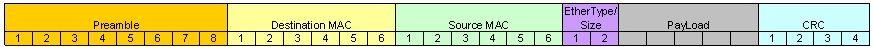
\includegraphics[width=16cm]{img/EthernetFrame.jpg}

\begin{description}
	\item[Präambel]: Zum Synchronisieren von Sender und Empfänger, \emph{Einschwingphase} (8 Byte)
	\item[SFD]: Festgelegte Sequenz 10101011 (1 Byte)
	\item[Ziel-Mac-Adresse]: Adresse des Empfängers (8 Byte)
	\item[Quell-Mac-Adresse]: Adresse des Senders (8 Byte)
	\item[VLAN-Tag]: Nach IEEE 802.1q, optional (4 Byte)
	\item[Typ-Feld]: Identifiziert die Art des nachfolgenden Inhalts, z.B. IP, ARP, etc...
	\item[Nutzlast]
	\item[PAD-Füllfeld]: Wird optional benötigt, um die Mindestlänge von 64 Byte einzuhalten \footnote{Rausfinden, warum mindestens 64 Byte nötig. Vermutung: Kollisionserkennung}
	\item[CRC-Prüfsumme]: Zur Fehlererkennung (4 Byte)
\end{description}

\subsubsection{CSMA/CD}

CSMA/CD regelt den Zugriff auf ein von mehreren Teilnehmern genutztes Medium (Kabel).
Dazu prüft der sendende Host, ob das Medium frei ist, bevor er sendet.
Beim Übertragen von Daten können Kollisionen erkannt werden.
Der Sendevorgang wird dann nach einer zufälligen Zeit wiederholt.
Aufgrund der verbreiteten Nutzung von Switches sind echte geteilte Medien inzwischen eher die Ausnahme.

$\Rightarrow$ Jeder Port am Switch bildet eine eigene \emph{Kollisionsdomäne}.
Die Bustopologie mit Koaxialkabeln (aber auch mit Hubs) wird nicht mehr genutzt.

\subsubsection{Duplex / Half Duplex}

Beim \textbf{Full Duplex} sind beide Seiten in der Lage, gleichzeitig zu Senden und zu Empfangen.
Im Falle von \textbf{Half Duplex} ist dies nur wechselseitig möglich (vgl Walkie Talkie).
Es sind verschiedene Realisierungen einer geteilten Nutzung eines Mediums möglich:

\begin{description}
	\item [Zeitduplex (TDD)]: Übertragung in verschiedenen Zeitschlitzen
	\item [Frequenzduplex (FDD)]: Übertragung auf verschiedenen Frequenzen
	\item [Codeduplex]: (nicht im Skript)
\end{description}

\subsection{Switching}

\textbf{Switches} sind Geräte auf dem OSI-Layer 2.
Sie empfangen Ethernet-Frames und leiten sie anhand ihrer Empfänger-MAC-Adresse weiter.
Im Gegensatz zum Hub wird dabei nur über den Port ausgegeben, hinter dem sich der Empfänger befindet.
Die Ausnahme ist hierbei, wenn der Port des Empfängers nicht bekannt ist.
Anhand der empfangenen Frames lernt ein Switch, wo sich Geräte befinden.

\subsubsection{Realisierungsmöglichkeiten}

%TODO Switches - Realisierungsmöglichkeiten

\subsubsection{Cut-Through und Store-and-Forward}

Beim \textbf{Cut-Through} (auch \emph{On The Fly Forwarding}) werden Pakete sofort nach Empfang der Empfängeradresse auf dem entsprechenden Port weitergeleitet, sofern dieser Frei ist.
Diese Methode ist sehr schnell (Verzögerung ca. 40$\mu$s), leitet jedoch gegebenenfalls auch fehlerhafte Frames weiter, da CRC umgangen wird.

\textbf{Store-and-Forward} hingegen empfängt zuerst den gesamten Frame, prüft diesen und leitet ihn anschließend weiter.
Offensichtlich werden keine fehlerhaften Pakete mehr in benachbarte Segmente weitergeleitet, dies wird jedoch durch erhöhte Latenz erkauft.

In der Praxis arbeiten Switches häufig im Cut-Through-Modus und schalten bei erhöhter Fehlerrate in den Store-and-Forward-Modus.

\subsubsection{VLAN}

Ermöglicht die Aufteilung von Switches in mehrere virtuelle LANs.
Den Ports werden dabei einzelne VLANs zugeordnet.
Auf diese Weise kann Hardware eingespart werden.
Realisiert wird dies mit einem 4 Byte langen Feld im Ethernet-Frame:
\begin{itemize}
	\item 2 Bytes \textbf{TPID} - Tag Protocol Identifier – Fester Wert 0x8100. Frame
	trägt die 802.1q/802.1p-Tag-Information
	\item 3 Bit \textbf{Priorität} (user\_priority) – Benutzer-Prioritätsinformationen
	\item 1 Bit \textbf{CFI} - Canonical Format Indicator – Gilt für alle vorhandenen
MAC-Adressinformationen im MAC-Datenpaket des Frames. Wert 0
das Format ist kanonisch (am wenigsten signifikante Bit zuerst); Wert
1 Format nicht-kanonisch. Benutzung im Token Ring/Source-Routed-
FDDI-Media-Zugang, um die Bit-Order der Adressinformationen des
verkapselten Frames festzulegen
	\item 12 Bit \textbf{VID} - VLAN Identifier – Identifizierung des VLANs zu dem der
Frame gehört
\end{itemize}
Erleichtert die Arbeit eines Administrators, da es viele Probleme von physikalischen Verbindungen umgeht. (bspw. Viel Hardware, unflexibel, Anpassungen nur mit hohem Aufwand)\\


\glqq Faulheit ist die Mutter der Ingenieurswissenschaften\grqq\\
\subsubsection{Trunking / Link Aggregation}
Ermöglicht die Zusammenfassung mehrerer Ports zur Erhöhung des Datensatzes.

\subsection{Asynchronous Transfer Mode}

\subsection{ATM}
	\begin{itemize}
		\item ATM kann als Protokoll für Internettelefonie eingesetzt werden und bietet eine geringe Latenz (von unter 200ms).
		\item Im Gegensatz zu Ethernet bietet ATM Garantien(!) und besitzt einen geringen Header von 5Byte. Es wird eine Leitung für den Datenstrom geschaltet.
		
	\end{itemize}

\subsection{Internet Protocol}
\label{subsec:ip}
Beim Internet Protocol handelt es sich um ein Layer-3-Protkoll, weches auf die Layer-2-Protokolle Ethernet, ATM und FDDI aufsetzen kann.
Es verwendet globale, logische Adressen.
Aufgrund der Erschöpfung des IPv4-Adressraumes\footnote{Weitere Maßnahmen, dem entgegenzuwirken sind etwa: NAT, CIDR, DHCP, Private Adressräume} (32 Bit) wird nach und nach IPv6 eingeführt (128 Bit)

\subsubsection{IPv4}
Wurde im RFC 791\cite{rfc791} definiert.
Der Header eines IPv4 Paketes ist insgesamt 20 Byte lang.
Davon sind insbesondere die folgenden von Interesse:

\begin{description}
	\item [Version]: In diesem Fall \emph{4}, bei IPv6 offensichtlich \emph{6} (4 Bit)
	\item [Header Length]: Gesamtlänge des Headers kann 20 Byte überschreiben, wenn zusätzliche Optionen gesetzt werden. Angabe in 32-Bit langen Blöcken (4 Bit)
	\item [Total Length]: Gesamtgröße des Pakets. Nach RFC muss jeder Host in der Lage sein, mindestens Pakete mit einer Länge von 576 Bytes zu verarbeiten. (16 Bit)
	\item [Type of Service]: Type of Service nach RFC791(ursprünglich für Quality-of-	Service-Anwendungen gedacht)
	
	\begin{itemize}
		\item bits 0-2: precedence
		\item bit 3: 0 = Normal Delay, 1 = Low Delay
		\item bit 4: 0 = Normal Throughput, 1 = High Throughput
		\item bit 5: 0 = Normal Reliability, 1 = High Reliability
		\item bits 6-7: Reserved for future use
	\end{itemize}
	Heute anders verwendet zur Servicebeschreibung durch Dienstklassen (DiffServ, 8 Bit)
	\item [Identification]: Falls ein Paket fragmentiert wird, haben alle Fragmente die	selbe Identification.
	\item [Flags]: Reserved\cite{rfc3514}, Don't Fragment, More Fragments (3 Bit)
	\item [Fragment Offset]: Kann ein Paket nicht auf einmal übertragen werden (z.B. bei
	kleinerer Maximum Transfer Unit, MTU), wird es fragmentiert.
	FO gibt an, ab welcher Stelle (gemessen in Blöcken von 8 Byte)
	dieses Paket die Daten enthält (MF Flag ist gesetzt) (13 Bit)
	\item[TTL]: Anzahl der Hops, bis Paket verworfen wird (wird bei jedem Routingvorgang reduziert)
	\item[Protocol]: Enthält für die darüber liegenden Layer Informationen, \glqq sodass diese etwas damit anfangen können\grqq
	\item[Checksum] wird selbst als 0 betrachtet, und fließt so nicht in die Kalkulation mit ein
	\item [Options]: Beispielsweise für Source Routing (Route ist im Paket vorgegeben); Sehr selten verwendet, häufig blockiert oder ignoriert
\end{description}

\begin{center}
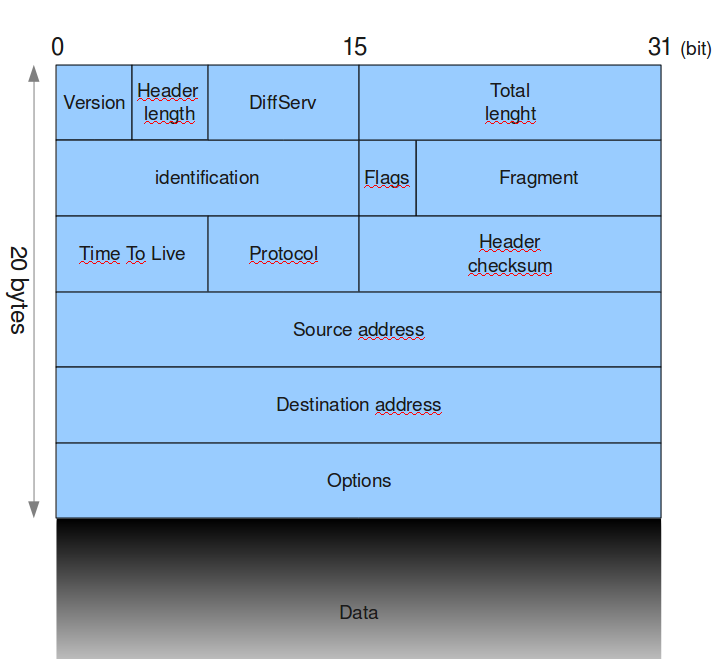
\includegraphics[width=8cm]{img/IP_packet}
\end{center}

Nutzung von Adressklassen\footnote{Class A 1.x.y.z-126.x.y.z; Class B 128.0.y.z-191.255.y.z; Class C 192.0.0.z-223.255.255.z} aufgrund der Verknappung der Adressen durch CIDR\cite{rfc1519} abgelöst.
Dies ermöglichte Super- und Subnetting.
Adressangabe bei CIDR im Format a.b.c.d/x, wobei x angibt, wie viele Bits zum Netz-Anteil der Adresse gehören.
Subnetze dienen zur Aufspaltung von Netzen in Teile, um diese besser handhaben zu können (Broadcast-Domains, Logische Strukturierung, Dezentrale Verwaltbarkeit)
\subsubsection{IPv6}

Die auffälligste Änderung von IPv4 zu IPv6 ist die vergrößerte Adressgröße (128 Bit).
Damit ergeben sich $3,4 \cdot 10^{38}$ Adressen.
IP - Adressen werden im Hexadezimalsystem zu je acht Word-Gruppen á 2 Bytes dargestellt.
Verkürzte Darstellung möglich durch Verzicht auf „Nullen“ in einer Gruppe (einmal je Adresse).
Es existieren IPv4-kompatible Adressen und die CIDR-Darstellung für Subnetze bleibt erhalten.
Weiterhin wurde die Anzahl der Felder im Header reduziert und (optionale) Erweiterungsheader hinzugefügt.
Wichtige Felder sind:

\begin{description}
	\item [Traffic Class]: \begin{itemize}
		\item 0 uncharakterisierter Verkehr
		\item 1 „Füllmaterial", z.B. Newsgroups
		\item 2 zeitunkritischer Verkehr, z.B. EMail
		\item 3 reserviert
		\item 4 Mengendaten, z.B. FTP, NFS
		\item 5 reserviert
		\item 6 Interaktive Anwendungen, z.B. telnet
		\item 7 Steuerung, z.B. SNMP
	\end{itemize}
	\item [Flow Label]: Anwendung kann Datenstrom mit einem Flow-Label versehen, z. B. bei Streaming-Anwendungen.
	Flow nicht notwendigerweise an Verbindung gebunden (logisch, da IP nicht verbindungsorientiert arbeitet).
	Empfänger kann Datenstrom am Flow Label erkennen. \cite{rfc3697, rfc6437}
	\item[Next Header]: Gibt an, dass ein weiterer Header folgt.
	In IPv6 sind viele Felder weggefallen.
	Next Header ermöglicht das Anfügen eines weiteren Headers.
	RFC 2460\cite{rfc2460} bietet beispielsweise:
	\begin{itemize}
		\item Hop – by – Hop Options Header
		\item Routing Header
		\item Fragmentation Header
		\item Authentication Header
		\item Encapsulated Security Payload (ESP) Header
		\item Destination – Option – Header
	\end{itemize}
	 
\end{description}

\begin{center}
	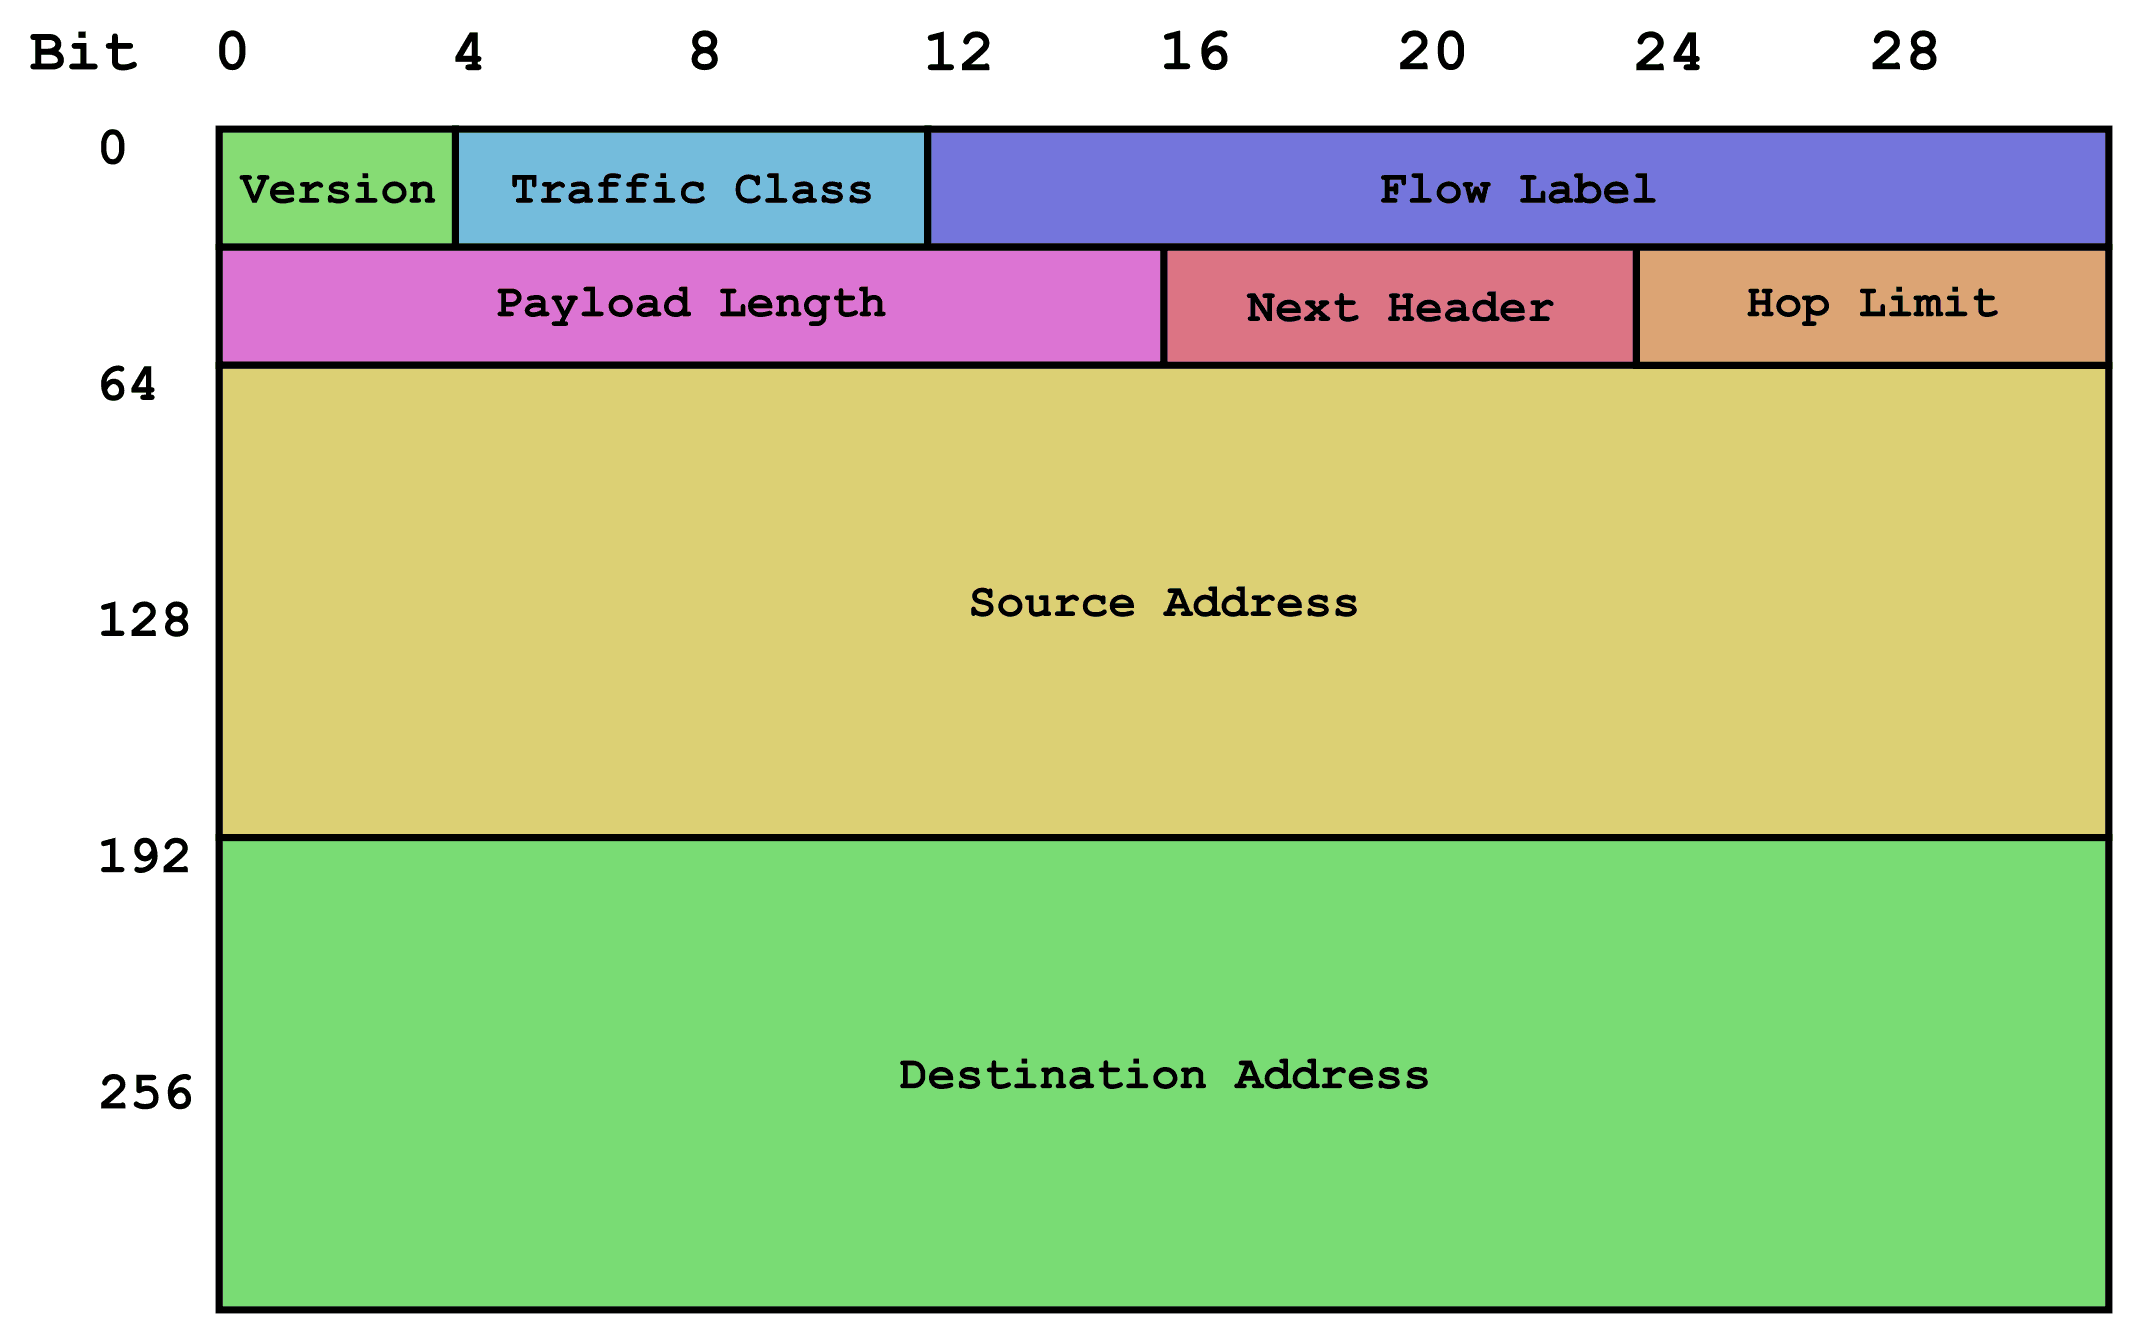
\includegraphics[width=10cm]{img/IPv6_header}
\end{center}

\subsubsection{Migration von IPv4 nach IPv6}

\emph{Wie migriert man Millionen von Hosts im Internet auf IPv6?}
Langsam, nach und nach.
Alle Hosts auf einmal sind nicht realisierbar.
RFC 1933\cite{rfc1933} schlägt drei Migrationsstrategien vor.

\begin{description}
	\item [Tunneling]: Zwischen zwei IPv6-Knoten wird ein virtueller Link aufgebaut.
	Die IPv6-Pakete werden (als Payload) in IPv4-Pakete verpackt und \emph{normal} über das Internet geroutet.
	\item [Dual Stack]: Auf Hosts und Routern werden sowohl IPv4 als acuh IPv6 eingerichtet.
	DNS kann A- oder AAAA-Records zurück geben, entsprechender Stack wird dann genutzt.
	%TODO Hier ist inhaltliche Überprüfung notwendig.
	Wird häufig mit Automatic Tunneling\footnote{\textquotedblleft IPv6-over-IPv4 tunneling where the IPv4 tunnel endpoint address is determined from the IPv4 address embedded in the IPv4-compatible destination address of the IPv6	packet.\textquotedblright} genutzt.
	
	Außerdem besteht die Möglichkeit von \textbf{Assignment of IPv4 Global Addresses to IPv6 Hosts} (AIIH).
	Dabei wird eine IPv4-kompatible IPv6-Adresse genutzt.
	Diese entspricht dem 96-bit Präfix 0:0:0:0:0:0, gefolgt von der IPv4-Adresse.
	Ist der Client der Dual-Stack-Hosts und der Server IPv4-only, verlangt der Client für die Dauer der Kommunikation eine	temporäre IPv4 Adresse beim AIIH Server (Kooperation von DNS und DHCPv6).
	Andernfalls (Client IPv4-only; Server Dual-Stack): DNS verlangt bei DHCPv6 eine temporäre IPv4 Adresse für Dual-Stack Host, welcher mit dieser rekonfiguriert wird.
	\item [Übersetzung der Header](Header Translation): Hierbei wird die IPv4 Unterstützung auf Systemen entfernt. Die IPv4-Pakete werden in IPv6-Pakete übersetzt; ein Translator übersetzt IP und ICMP Meldungen.
	%TODO Ist mit den Erweiterungsheadern das Options-Zeugs bei IPv4 gemeint?
	Erweiterungsheader werden nicht, oder nur bedingt übersetzt.
	Probleme entstehen, weil sich einige Felder nicht immer übersetzen lassen und Adressumwandlung Datenbanken-Lookups erfordern.
\end{description}


\subsection{User Datagram Protocol}

Bei UDP handelt es sich um ein Layer-4-Protokoll.\cite{rfc768}
Es dient zur Übermittlung kurzer Nachrichten an andere Systeme und garantiert weder Zuverlässigkeit noch Einhaltung der Reihenfolge der Pakete beim Empfänger.
Die Adressierung geschieht über Ports (16 Bit).
Der Header enthält 4 Felder (je 16 Bit): Quellport, Zielport, Datagram-Länge und eine Checksumme.

\subsection{Transmission Control Protocol}

TCP ist ebenfalls ein Layer-4-Protokoll.\cite{rfc793}
Es garantiert eine Ankunft der Pakete in korrekter Reihenfolge.
Clienten sehen die Verbindung als bidirektionalen Datenstrom, tatsächlich findet die Kommunikation über Pakete statt. Die Kommunikation erfolgt durch TCP zustandsbehaftet.

\subsubsection{Paketstruktur}

Der Header des TCP-Fragments ist 20 Byte groß.
Wichtige Felder sind:
\begin{description}
	\item [Sequence Number / Acknowledgement Number]: Zerlegung des Datenstroms in nummerierte Blöcke.
	Größe der Blöcke ist variabel (Nagle Algorithmus).
	Verwerfen von Segmenten mit fehlerhafter Prüfsumme.
	Bestätigung empfangener Segmente.
	Nicht unbedingt für jedes Segment einzeln (Windowing).
	Erneuter Transport unbestätigter Segmente.
	Zusammensetzung des Datenstroms auf Empfängerseite
	
	\item [Flags]: dienen unter anderem zur Steuerung des Verbindungsauf- und –abbaus.
	\begin{description}
		\item [URG] - Urgent Flag (Urgent Pointer enthält
			Sequenznummer, die bevorzugt übertragen werden soll)
		\item [ACK] – Acknowledgement
		\item [PSH] – Push (Paket wird sofort an Anwendung weitergeleitet, ohne Zwischenpuffer)
		\item [RST] – Reset (Unterbrechung der Verbindung)
		\item [SYN] – Synchronized (Aufbau der Verbindung)
		\item [FIN] – Finish (Beenden der Verbindung)
	\end{description}
	\item [Window Size]: Anzahl der Daten, die gesendet werden können bis ein Acknowledgement gesendet werden muss (in Bytes oder mit speziellem Option Header nach RFC1323 \cite{rfc1323} auch bis zu 1GB,	dann Linksverschiebung um bis zu 14 Bits, $2^{14} \cdot 64k = 1G$).
\end{description}

\subsubsection{Zustände}

Zum Aufbau einer Verbindung wird der \textbf{3-Way-Handshake} durchgeführt:
\begin{enumerate}
	\item $\rightarrow$ SYN
	\item $\leftarrow$ SYN + ACK
	\item $\rightarrow$ ACK
\end{enumerate}
Ein Timeout findet typischerweise nach 75 Sekunden statt. Zum Abbau der Verbindung genügt das Senden und Quittieren eines FIN.

\subsubsection{Sliding Window}
%TODO
\subsubsection{Nagel-Algorithmus}
%TODO
\section{Adressierung}

% 030
\subsection{MAC-Adressen}

\begin{itemize}
	\item Layer-2-Adressen für Ethernet
	\item 6 Byte / 48 Bit groß
	\item \emph{Eigentlich} weltweit eindeutig
	\item \emph{Eigentlich} in Hardware gegossen, trotzdem fälschbar
	\item Darstellung: Hexadezimal, Bits getrennt durch \[.:-\]
	\item Bit 3 bis Bit 24 an Hersteller gebunden (z.B. 00-60-2F-xx-xx-xx für Cisco)
	\item Broadcast: FF-FF-FF-FF-FF-FF 
\end{itemize}

\subsection{VPI und VCI bei ATM}

%TODO VIP und VPI bei ATM

\subsection{IP-Adressen}

Siehe Abschnitt \ref{subsec:ip}.

\subsection{Ports}

Für die Layer-4-Protokolle UDP und TCP werden 16-Bit-Adressen verwendet.
Diese werden als Ports bezeichnet.
Ports 0-1023 sind dabei standardisiert.
Wichtige Portnummern sind beispielsweise:
\begin{center}
\begin{tabular}{|c|c|c|c|}
	\hline Port & TCP & UDP & Beschreibung \\ 
	\hline 20 & Ja & Nein & FTP - Datenübertragung \\ 
	\hline 21 & Ja & Nein & FTP - Kontrolle \\ 
	\hline 22 & Ja & (Ja) & SSH \\ 
	\hline 23 & Ja & Nein & Telnet \\ 
	\hline 25 & Ja & Nein & SMTP \\ 
	\hline 53 & Ja & Ja & DNS \\ 
	\hline 80 & Ja & Nein & HTTP \\ 
	\hline 110 & Ja & Nein & POP3 \\ 
	\hline 123 & Nein & Ja & NTP \\ 
	\hline 443 & Ja & Nein & HTTPS \\ 
	\hline 
\end{tabular} 
\end{center}
\subsection{URIs, URNs und URLs}
\begin{description}
\item [Uniform Resource Identifier]: String; Benennt oder identifiziert eine Ressource z.B.  \textbackslash\textbackslash139.30.3.23\textbackslash iukp\textbackslash beispiel.txt
\item [Uniform Resource Name]: Sonderform der URI, die eine Ressource in einem bestimmten
Namespace benennt | urn:ip-addr:139.30.3.23
\item [Uniform Resource Locator]: Sonderform der URI, die zusätzlich das Protokoll angibt, über das die Ressource erreichbar ist z.B. http://139.30.3.23/beispiel.txt
\end{description}
\subsection{*cast} 
\begin{description}
	\item[Unicast]: Einer sendet an einen, wie beispielsweise in einer TCP-Verbindung für HTTP. Adressierung durch Angabe des Empfängers.
	\item[Broadcast]: Einer sendet an alle, wie beispielsweise in ARP oder DHCP. Hierzu werden spezielle Adressen (MAC: FF-FF-FF-FF-FF-FF; IP: höchste Adresse im Subnetz) verwendet. Broadcastbereiche sollten möglichst klein gehalten werden, um möglichst wenig Teilnehmer zu belästigen.
	\item[Multicast]: Einer sendet an viele Mitglieder einer Gruppe. Siehe Abschnitt \ref{sec:muliticast}.
	\item[Concast]: Viele senden an einen, Nachrichten werden so früh wie möglich zusammengefasst. Verhindert Implosion, Überlastung des Empfängers. Beispielswiese sinnvoll, wenn Fehlermeldungen zusammengefasst werden können. Keine direkte Unterstützung in IP, MAC, Ethernet
\end{description}

%TODO Foliensatz enthält noch ICMPv6 Neighbor Discovery Protocol, Domainverwaltung und Domain Registry
\section{ARP, RARP}

% Ende 030, 040

ARP wandelt Layer-3-Adressen in Layer-2-Adressen um.
Es beschränkt sich nicht auf das Erfragen von MAC-Adressen zu IP-Adressen, sondern ermöglicht beispielsweise auch ATM ARP, IP over FDDI und IP over Token Ring.
\begin{itemize}
	\item Erfragt für gegebene IP-Adresse eine MAC-Adresse.
	\item Host erzeugt Broadcast.
	\item Der angefragte Host darf darauf antworten (Unicast).
	\item Nachdem der Sender der Broadcast-Nachricht die Antwort erhalten hat, kann er die IP-Adresse der Ethernet-Adresse zuordnen.
	\item Diese Ethernet-Adresse wird dann für alle folgenden Pakete an diese Internet-Adresse verwendet, solange bis die Cache-Zeit abgelaufen ist.
	\item RFC 826 \cite{rfc826}
\end{itemize}

\subsection{Einsatzfälle}

\begin{enumerate}
	\item Zwei Hosts möchten im selben Netzwerk (ausschließlich Layer 2) miteinander kommunizieren und kennen nur die Layer-3-Adresse (z.B. IP-Adresse) des Empfängers.
	\item Ein Host benötigt die Layer-2-Adresse des Gateways, um andere Netze zu erreichen (Sonderfall des zuvor genannten)
	\item Zwei Gateways wollen kommunizieren.
\end{enumerate}

\subsection{Paketstruktur}
Wichtige Felder eines ARP-Requests sind:
\begin{description}
	\item[Hardware type]: Kennzeichen für die verwendeten Hardware-Adressen (1 für Ethernet, 2 Byte)
	\item[Protocol type]: Kennzeichen für die verwendeten Protokoll-Adressen (L3) (0x0800 für IPv4, 2 Byte).
	\item[Hardware length]: Länge der Hardware-Adresse in Bytes (6 für Ethernet, 1 Byte)
	\item[Protocol Length]: Länge der Protokoll-Adressen (L3) (4 für IPv4, 1 Byte)
	\item[Operation]: Unterscheidung von 1 Request und 2 Reply, da für beides gleiche Pakete verwendet werden (2 Byte, warum zur Hölle reserviert man für 2 Werte 2 Byte?)
\end{description}

Es folgen Sender hardware address, Sender protocol address, Target hardware address und Target protocol address

\subsection{ARP-Caching}

Um nicht für jedes IP-Paket einen neuen ARP Request zu stellen, werden die Ergebnisse zwischengespeichert.
Typischerweise 10 Minuten lang.
Kommt es während der Cache-Zeit zu einem Fehler (Host nicht erreichbar), wird erneut ein ARP-Request ausgeführt.

\subsection{ARP-Announcements}

Der anfragende Host sendet bekanntlich einen Broadcast, alle Host im gleichen Netz können folglich diese Information ebenfalls verwenden, und auf diese Weise eigene Anfragen sparen.
Anwendungen:
\begin{itemize}
\item Unterbrechungslose Übernahme einer Protokoll-Adresse (z.B. IP-Adresse) in hochverfügbaren Systemen.
\item Der anfragende Host kann auf diese Weise feststellen, ob eine Protokoll-Adresse bereits vergeben ist (Gratuitous ARP). Dieser Mechanismus wird bei IP-Autoconf verwendet.
\end{itemize}

IP-Autoconf \cite{rfc3927} ist eine einfache Möglichkeit zur Adresskonfiguration ohne Server (DHCP, RARP).

\begin{itemize}
	\item Host wählt zufällig eine Adresse.
	\item Überprüft mittels Gratuitous ARP, ob diese Adresse bereits vergeben ist.
	\item Falls ja, andere Adresse zufällig wählen und erneut überprüfen.
	\item Falls nein, Adresse benutzen und andere ARP Requests für diese Adresse beantworten.
\end{itemize}

\subsection{ARP-Spoofing}

Da ARP nicht kryptografisch abgesichert ist, kann jeder Host auf ARP Requests antworten oder ARP Announcements erzeugen.
Ziel ist das Umleiten von Datenpaketen.
Es gibt Programme, die Änderungen der Hardware-Adressen erkennen (z.B. arpwatch).
Der Administrator muss dann die Ursache überprüfen

\subsection{Proxy ARP}

Wird von speziellen Routing-Protokollen verwendet.
Jeder Nachbar (One-Hop-Neighbor), der auf der Route zum Ziel liegt, beantwortet einen eintreffenden ARP-Request mit seiner Hardware-Adresse.
Pakete werden so von Host zu Host weitergeleitet

\subsection{Reverse RP}

Erfragt eine IP-Adresse bei bekannter MAC-Adresse und ist nicht unbedingt für die Funktionsfähigkeit von IP über Ethernet notwendig.
RARP wird in RFC 903 \cite{rfc903} standardisiert.
Haupteinsatzzweck ist die automatische Konfiguration der Protokoll-Adresse.
Dabei sendet der Host einen RARP-Request mit der eigenen Hardware-Adresse (z.B. MAC).
Ein RARP-Server beantwortet diesen Request und liefert die hinterlegte Protokoll-Adresse (z.B.IP).
Da RARP Link-Local-Broadcasts verwendet, ist ein RARP-Server pro Netz notwendig.
Benutzt gleiche Paketstruktur wie ARP, lediglich anderen EtherType\footnote{Feld im Ethernet-Header, siehe Abschnitt \ref{subsec:ethernet}} (0x8035)

\section{DNS und WHOIS}

% 050
%TODO Ordnung in die Informationen bringen. Folien haben keinen guten roten Faden
Die Aufgabe des Domain Name Systems ist die Übersetzung von (Layer-4) IP-Adressen in, für den menschlichen Gebrauch besser verwendbare Namen.
Der Name wird dabei aus hierarchischen Domains, getrennt durch Punkte (.) zusammengesetzt.\\
Direkt unter der Wurzel steht hierbei die sogenannte Top-Level-Domain.
Bei Top-Level-Domains wird zwischen \textbf{länderspezifischen} (ccTLD) und \textbf{generischen} (gTLD) Domains unterschieden.
Während erstere, bestehend aus zwei Buchstaben, durch lokal verantwortliche Institutionen\footnote{Network Information Centers z.B. DENIC für .de} verwaltet werden, werden gTLD durch die \textbf{ICANN} oder beauftragte Institutionen vergeben.
%TODO 050_DNS.pdf hat hier noch so eine komische Seite 61
Bei der Vergabe gilt das \emph{first come, first serve}-Prinzip.
Für die Namensbildung gelten gewisse Regelungen, z.B. Ziffern 0-9, Bindestriche, Buchstaben, sowie einige ausgewählte lokale Buchstaben.
Letztere müssen ASCII-kodierbar sein (ACE)\cite{rfc3490}.
Jede (Teil-) Domain ist maximal 63 Zeichen lang, insgesamt ist der vollständige Pfad jedoch 255 Zeichen lang.
Folgende Daten sind bei der Domainanmeldung von Interesse:

\begin{description}
	\item[Domaininhaber](Holder): Person, der die Domain \emph{gehört}
	\item[Administrativer Ansprechpartner]: Vom Inhaber Bevollmächtiger, darf alle Entscheidungen treffen (Admin-C)
	\item[Technischer Ansprechpartner, Zonenverwalter]: Typischerweise Kontaktadresse der Firma, die die Domain betreibt (Tech-C, Zone-C)
	\item [Technische Daten]: z.B. Nameserver
\end{description}

Hoster tragen oft nicht den Inhaber selbst als Admin-C, sondern sich selbst ein.
Außerdem stellen sie in der Regel den Nameserver zur Verfügung.
Die Registrierung einer Domain gilt immer für einen bestimmten Zeitraum.
Ein Wechsel erfordert eine Freigabe beim alten Provider durch Inhaber oder Admin-C.

\subsection{Weiteres Bla zu DNS}

Beim Domain Name System handelt es sich um ein \textbf{sehr großes}, \textbf{hierarchisch strukturiertes}, \textbf{verteiltes}, \textbf{repliziertes} und \textbf{lokal verwaltetes System} \cite{rfc1034,rfc1035}.
Aus dem hierarchischen Benennungsschema resultiert das verteilte Datenbanksystem des DNS.
Jede Domain bestimmt selbst, wie die unter ihr liegenden Domains zugewiesen werden, hat dementsprechend eigene Verantwortlichkeiten.
Ist ein Namensserver für eine solche Zone verantwortlich, kann er Anfragen autoritativ beantworten(Autoritäskonzept).
Andernfalls wird die Anfrage aus dem Cache beantwortet oder an einen anderen Nameserver delegiert (Delegationskonzept).
Das kann der Nameserver einer Subdomain oder (default) ein Root Name server sein.\\
Die Aufteilung in die Zonen erfolgt anhand von Punkten - Bsp: www.spiegel.de

\subsection{Servertypen}

\begin{description}
\item[Primary Server]: Ist Hauptserver einer Domain und autorisiert, Anfragen zu seiner Domain verbindlich zu
beantworten.
Er verfügt über alle Daten dieser Domain, welche in Zonen-Dateien abgelegt sind, die der Verwalter des
Servers erstellt
\item[Secondary Server]: Ist ebenfalls autorisiert, verbindliche Antworten zu seiner
Domain zu liefern, lädt die Domain-Datenbank von einem Primary Server und aktualisiert sie bei Bedarf
\item[Caching-only Server]: Verfügt über keine eigenen Domain-Informationen.
Fragt bei dem für die Domain zuständigen Primary oder Secondary Server nach und speichert die Antwort zwischen.
Ist zur Beantwortung von Anfragen zu einer Domain „nicht autorisiert“ (kann die Genauigkeit und Aktualität nicht gewährleisten)
\item[Slave	Server]: Reicht alle Anfragen, die er selbst nicht aus seinem eigenen Cache beantworten kann, an eine zuvor festgelegte Liste von anderen Servern (Forwarders) weiter.
Forwarders fragen ihrerseits den zuständigen Server und speichern Ergebnis zwischen (Caching)
\end{description}

%TODO DNS ist noch nicht fertig


\section{Timeouts, ACK, Bestätigungen}

% 070
%TODO Timeouts, ACK, Bestätigungen

\section{Routingkonzepte}

% 080, 090, 095, 100, 110, 120, 130
%TODO Routingkonzepte

\subsection{Begriffe}

\subsection{Routing-Algorithmen}
%Anforderungen
%Djikstra
%Bellman-Ford

\subsection{Link-State-Routing}

\subsection{Distance-Vector-Routing}

\subsubsection{Count-to-infinity-Problem}

\subsection{Routing in MANETs}

\section{Quality of Service}
\label{sec:qos}
% 140
%TODO Quality of Service

\section{Multicast}
\label{sec:muliticast}
% 150, 180
%TODO Multicast

\section{Zeitsynchronisation}

% 160, 190

\subsection{Notwendigkeit der Zeitsynchronisation}
Authentisierungsverfahren müssen die Gültigkeit von Schlüsseln überprüfen können.
Ebenso haben einige Abläufe eine beschränkte zeitliche Dauer.
Andere Verfahren benötigen Time-Stamps, Vorher-Nachher-Beziehungen von Ereignissen müssen bekannt sein.

Uhren in verteilten Systemen sind nicht zwangsweise synchron.
Sie können unterschiedliche Zeiten aufweisen, je nach Art der Uhr \emph{ticken} sie unterschiedlich schnell (Quarzuhr, Atomuhr).
Zusätzlich kann die physikalische Umgebung diesen Effekt verstärken (z.B. Temperatur einer Quarzuhr).
Eigenschaften von Uhren nach Mühl sind: Drift, Auflösung und Abweichung (von der Realzeit).

\subsection{Logische Zeit}
Manchmal reicht es, nicht den genauen Zeitpunkt von Ereignissen, sondern lediglich die Vorher-Nachher-Beziehung zu kennen.
Man spricht von \textbf{Lamport-Zeitstempel} oder \textbf{Vektoruhren}.
Empfangene Lamport-Zeitstempel werden einfach bei jedem Kommunikationsschritt um eins inkrementiert und dann als eigener Zeitstempel versendet.
Bei der Vektor-Zeit werden zusätzlich die Zeitstempel der anderen Kommunikationspartner mitgeführt.
Dies hat den Vorteil, dass ein kausaler Zusammenhang immer erkennbar ist.

\subsection{Herausforderungen}
\begin{itemize}
	\item Logische Zeitstempel (Lamport-Zeitstempel und Vektor-Zeit) genügen den Anforderungen nicht immer.
	\item Viele Uhren müssen synchronisiert werden.
	\item Die Übertragung eines Zeitstempels kostet Zeit – Latenz.
	\item Die Latenz ist nicht konstant – Jitter.
	\item Die Latenz ist nicht symmetrisch.
\end{itemize}

\subsection{Algorithmen}
\textbf{Anforderungen} an Algorithmen sind symmetrische oder bekannte Laufzeiten und eine konstante Latenz.
Letzteres ist in paketvermittelnden Netzen nicht erreichbar.
\subsubsection{Algorithmus von Cristian}
Clients fragen beim Server nach der korrekten Zeit.
Server kennt die Zeit aus zuverlässiger, externer Quelle.

\subsubsection{Berkeley-Algorithmus}
Server fragt alle verfügbaren Clients nach der Zeit und bildet den Mittelwert.
Zeit wird anschließend an Clients verbreitet.

\subsubsection{Marzullo's Algorithmus}
Versucht den Einfluss des Jitters durch mehrfache Messungen zu eliminieren.
Messungen werden solange durchgeführt, bis das Konfidenzinterval den Anforderungen entspricht.

\subsection{NTP}
NTP\cite{rfc1305, rfc5905} verwendet Marzullo's Algorithmus.
Es löste den ICMP Timestamp Request (Abschnitt \ref{subsec:icmptime}) ab und ist mittlerweile in Version 4 aktuell.
NTP-Server lauschen auf UDP-Port 123.
Im Internet sind Genauigkeiten von $\leq 10ms$ erreichbar.

\subsubsection{Paketaufbau}
\textbf{Anmerkung}: Paketaufbau von Version 4 scheint sich recht stark von Version 3 zu unterscheiden.
Ich bleibe bei der in der Vorlesung besprochenen Version 3.
\begin{description}
	\item[Leap Indicator]: Gibt an, ob Schaltsekunde in dieser Minute hinzugefügt oder entfernt wird  (2 Bit)
	\item[Status]: Gibt mögiche Fehler an.
		\begin{enumerate}
			\setcounter{enumi}{-1}
			\item clock operating correctly
			\item carrier loss
			\item synch loss
			\item format error
			\item interface (Type 1) or link (Type 2) failure
		\end{enumerate}
	\item[Type]: Typ\footnote{Neuere Versionen bezeichnen dies als Stratum; Es gibt quasi eine Hierarchie bei den (Genauigkeiten der) NTP-Server} der Referenzuhr: 1 | Primärreferenz (z.B. Atomuhr) bis 4 | \emph{Eyeball and wrist watch}
	\item[Precision]: Angabe der Genauigkeit der Uhr (als Exponent zur Basis 2)
	\item[Estimated Error]: Geschätzter Fehler zum Zeitpunkt der Synchronisation in Sekunden.
	\item[Estimated Drift Rate]: Geschätzte Drift der Uhr (ohne Einheit).
	\item[Reference Timestamp]: Zeit, auf den die Uhr bei der letzten Synchronisation eingestellt
	wurde.
	\item[Originate Timestamp]: Zeit beim Senden des Pakets
	\item[Receive Timestamp]: Lokale Zeit bei Ankunft des Pakets
	\item[Transmit Timestamp]: Lokale Zeit beim Senden der Anwort
\end{description}

\subsection{SNTP}
Vereinfachung von NTP, bei der auf eine Wiederholung der Zeitsynchronisation verzichtet wird.
So sind etwa Synchronisationen über Multi- und Broadcasts möglich.
Es werden dasselbe Nachrichtenformat und derselbe UDP-Port, wie bei NTP genutzt\cite{rfc4330}.

\subsection{ICMP - Timestamp Request und Reply}
\label{subsec:icmptime}

Timestamp Request\cite{rfc792} ermöglicht die Anfrage eines anderen Systems nach der aktuellen Zeit.
Es handelt sich um ICMP-Nachrichten mit den Type-Werten 13 (Request) oder 14 (Reply)\footnote{Skript sagt hier 17 und 18, im RFC stehen allerdings 13 und 14. Habe Thomas drauf hingewiesen.}.
Empfohlener Rückgabewert sind die Millisekunden seit Mitternacht (Coordinated Universal Time - UTC).
ICMP-Data-Bereich kennt Felder \textbf{Originate Timestamp}, \textbf{Receive Timestamp} und \textbf{Transmit Timestamp} (je 32 Bit); diese scheinen dieselbe Bedeutung wie bei NTP zu haben.
Außerdem \textbf{Identifier} und \textbf{Sequence Number}, diese gestatten dem Sender eine Zuordnung von Replies bei mehreren Requests.
Letztere werden vom Sender eingetragen und vom Empfänger in die Antwort kopiert.

\section{Internet Control Message Protocol}

ICMP ist ein Layer-3-Protokoll zur Steuerung des Nachrichtenaustausches im Internet\cite{rfc792}\footnote{Laut Folien RFC 950\cite{rfc950}, aber das ist Quatsch (\emph{Internet Standard Subnetting Procedure})}.
Es dient häuptsächlich dem Austausch von Status- und Fehlermeldungen zwischen Gateways und Hosts.
Die Nachrichten werden über IP-Datagramme übertragen, das Protokoll ist verbindungslos.

\subsection{Paketaufbau}
Eine ICMP-Nachricht besteht aus den Feldern \textbf{Type}, \textbf{Code}, \textbf{Checksum} und \textbf{Data}, angeführt von einem 20 Byte IP-Header.
Der IP-Header hat häufig vorbestimmte Feldwerte, z.B. Type of Service = 0, weitere Infos im RFC.

\begin{description}
	\item[Type]: Bestimmt das Format der weiteren  Felder. (1 Byte)
	\item[Code]: Inhalt Abhängig vom Type (1 Byte)
	\item[Checksum]: Prüfsumme\footnote{Scheinbar abhängig vom Type; häufig: \emph{The checksum is the 16-bit ones's complement of the one's complement sum of the ICMP message starting with the ICMP Type.}} (2 Byte) 
	\item[Data]: Nicht immer genutzt; Enthält beispielsweise bei Type \emph{Redirect Message} (5) die \emph{Gateway Internet Address} oder die in Abschnitt \ref{subsec:icmptime} beschriebenen Felder für Timestamps.
\end{description}

\subsection{Beispiele}
Im Skript existiert eine umfangreiche Tabelle von Funktionen und entsprechender Werte für Type- und Code-Felder.
Diese auswendig zu lernen entspräche nicht 80-20.
Daher beschränke ich mich hier nur auf zwei Beispiele (+ Zeitsynchronisation in Abschnitt \ref{subsec:icmptime})

\subsubsection{Destination Unreachable}
Wird beispielsweise gesendet, wenn er Empfänger laut den Routing-Tabellen eines Gateways nicht erreichbar ist, z.B. weil die Distanz zum Zielnetzwerk unendlich ist.
Empfänger im IP-Header ist der ursprüngliche Absender einer (nicht zustellbaren) Nachricht.
Der ICMP-\textbf{Type} ist 3, der Code gibt genauere Informationen zur Fehlerursache (z.B. 3 | port unreachable)
\subsubsection{Ping}
Beispiel nicht aus dem Skript.
Beim Request wird ein \textbf{Echo-Request} (Type 8) versendet.
Das Feld \textbf{Code} enthält den Wert 0\footnote{Laut RFC scheint die Möglichkeit zu bestehen, dass hier etwas anderes steht. Warum das so ist, kann ich allerdings nicht finden}.
\textbf{Identifier} und \textbf{Sequence Number} helfen bei Unterscheidung mehrerer Requests/Replys.
Im \textbf{Data} Feld kann scheinbar noch unbestimmter Payload mitgesendet werden.

Bei der Antwort werden Sender- und Empfängeradresse im IP-Header vertauscht.
Der \textbf{Type} ist 0 (Echo-Reply).
Weitere Felder werden aus dem Request übernommen.

\subsection{Regeln}
ICMP-Fehler-Nachrichten werden nie als Folge auf
\begin{itemize}
\item  eine ICMP Fehlermeldung („Teufelskreislauf“) erzeugt.
\item  ein Datagram, das an eine IP Broadcast Adresse oder eine IP
Multicast - Adresse (class D) gesendet wird, erzeugt.
\item  ein Datagram, welches als Link - Layer Broadcast gesendet
wird, erzeugt.
\item  ein anderes Fragment als des ersten erzeugt.
\item  ein Paket erzeugt, dessen Quelladresse nicht einen einzelnen Host definiert.
\end{itemize}


\section{Internet Group Message Protocol}
%TODO Ist in Mitschriften genannt worden

\section{Voice over IP}

% 200, 210
%TODO Voip
\section{World Wide Web und HTTP}

% 220, 230
%TODO WWW und HTTP

Durchbruch des Internets erfolgte erst nach dem Erscheinen des ersten graphischen WWW-Browsers (\glqq Mosaic\grqq).
Dieser ermöglichte erstmals den komfortablen und effizienten Zugriff auf die Ressourcen des Internets.
Das zuvor \glqq beliebte\grqq{\ }Gopher wurde relativ schnell verdrängt.
Bis zum Ende der 90er-Jahre vervielfachte sich die Zahl der Websites dramatisch (1993 ca. 50; 1994 ca. 800, 2000 über 22 Millionen)

\subsection{Anforderungen an Internet-Protokolle}

\begin{itemize}
	\item Weitestgehende Unabhängigkeit von der Netzwerk-Hardware.
	\begin{itemize}
		\item Übertragungsmedium (Kupferkabel, Lichtwellenleiter usw.)
		\item Typ des lokalen Netzwerks (Ethernet, Token Ring usw.)
	\end{itemize}
	\item Erreichbarkeit aller Rechner im gesamten Internet.
	\item Fehlererkennung und Fehlerkorrektur.
	\item Logische Adressierung (Adresse eines Rechners sollte nicht von der Netzwerk-Hardware abhängen, da bei Defekt einer Ethernet-Karte beispielsweise eine ausgetauschte Karte zu einem Adresswechsel führen würde).
	\item Verbindungsherstellung.
	\item Datenübertragung (Versendung von Datenpaketen /Datagrammen).
\end{itemize}

\subsection{Hypertext Transfer Protocol}

HTTP wurde in RFC 2616\cite{rfc2616} definiert.
TLS\cite{rfc2817} führte später einige Sicherheitsfeatures ein.
Trotz des \emph{Hypertext} im Namen ist es generisch und ermöglicht die Übertragung beliebiger Inhalte.
HTTP ist \textbf{zustandslos} und nutzt den TCP-Port 80.
Es handelt sich um ein \textbf{Request-Response-Protokoll}.
Zusätzlich werden Nachrichten im ASCII-Klartext gesendet, solange sie nicht verschlüsselt werden.
Ressourcen werden über URIs\cite{rfc2396} adressiert.\footnote{Angeführt durch die Protokollangabe http:// oder https://, dabei handelt es sich dann allerdings um eine URL.}

Eine einfachste Anfrage an den Server wäre beispielsweise \ttfamily{GET index.html HTTP/1.1}.
Hierbei handelt es sich offensichtlich um eine Bitte, die Datei index.html auszuliefern und dabei HTTP 1.1 zu verwenden.

\subsection{File Transfer Protocol}

\section{Peer-to-Peer}

% 240, 250
%TODO P2P

\section{E-Mail}

% 260
%TODO Mail

\section{Autokonfiguration}

% 280, 290
%TODO Autoconfiguration

\section{Dateien und Drucken}

% 300, 310
%TODO Dateien und Drucken

\section{Telnet, SSH und rlogin}

% 320
%TODO SSH

\section{Extensible Messaging and Presence Protocol (XMPP)}

% 330
%TODO XMPP

\section{LDAP}

% 340
%TODO LDAP

\section{Authentication Protocols}

% 350
%TODO Authentication Protocols

\section{Simple Network Management Protocol}

% 360
%TODO SNMP 

\section{Mac-Sublayer}

% 365
%TODO Mac-Sublayer

\section{Mobile Netzwerke}

% 370, 380, 390, 400
%TODO Mobile Netzwerke

\section{HTTP2 und SCTP}

% 410
%TODO HTTP2, SCTP

\section{Thomas Fragestunde}
\subsection{08.04}
	\begin{itemize}
		\item Merkmale von Verbindungen
		\begin{enumerate}
			\item Latenz
			\item Datenrate
			\item Jitter\\
			(Änderung der Latenz über die Zeit)
			\item Verfügbarkeit
			\item Fehlerrate
		\end{enumerate}
		\item Bandbreite wird in Hz und nicht in Mbit/s angegeben (Wlan bspw.)
		\item Ursachen für Jitter
			\begin{itemize}
				\item Es ist notwendig zu warten, bis gesendet werden kann
				\item Sich ändernde Routen, durch bspw. Wegänderungen, Datenaufteilung durch den Router
				\item Zeit, Route, Warteschlangenproblematik, gemeinsam genutzte Medien, CSMA
			\end{itemize}
		\item Warum Begrenzung der Übertragungsraten?
			\begin{itemize}
				\item Physikalisch - Frequenzen
			\end{itemize}
		\item Was begrenzt den max. Durchsatz eines Glasfaseranschlusses
			\begin{itemize}
				\item unterschiedlich lange Wege
				\item Kapazität (Zeit bis Ladung angekommen ist)
				\item Transistoren schalten nicht so schnell
				\item Signal-Rausch-Verhältnis
			\end{itemize}
	\end{itemize}
\subsection{09.04}
	\begin{itemize}
		\item Was begrenzt die Bandbreite?
			\begin{itemize}
				\item Kapazität $\rightarrow$ Grenzfrequenz
			\end{itemize}			
		\item CSACD
			\begin{itemize}
				\item Warten auf freies Medium
				\item Es gibt jedoch keine Garantien
				\item Verursacht Jitter
			\end{itemize}
		\item Jitter Gegenmaßnahmen
			\begin{itemize}
				\item Puffer (Warteschlange, FiFo)
				\item Pakete werden in gleichmäßiger Reihenfolge erhalten
			\end{itemize}
		\item Leitungs- vs. Paketorientiert
			\begin{itemize}
				\item ?
			\end{itemize}
		\item Möglichkeiten zur Beschreibung eines Standards
			\begin{itemize}
				\item textuell (schwer)
				\item Referenzimplementation (bspw. Bittorrent - aber berücksichtigt ggf. nicht alle Fälle)
				\item Automaten (5-Tupel, Mealy/Moore)
			\end{itemize}
		\item Zustandsbehaftete und zustandslose Protokolle
			\begin{itemize}
				\item Beispiel TCP (closed, SYN, etc.) besitzt einen Zustand
				\item Ein Zustand merkt sich die \glqq Vorgeschichte \grqq und damit was passiert ist. Somit ist ein Login immer zustandsbehaftet.
				\item Werden die Zwischenschritte nicht gespeichert, ist es zustandslos.
				\item Cookies bieten die Möglichkeit einen Zustand nachzurüsten.
			\end{itemize}
		\item Autonome Systeme sind \glqq Provider \grqq, die miteinander über \textit{Peering Points} verbunden sind
		\item Minimierung der Aufreihungslatenz
			\begin{itemize}
				\item Entsteht dadurch, dass das Paket erst versendet wird, wenn es vollständig da ist
				\item Lösung, Weiterleiten, sobald die ersten 6 Byte (Adresse) bekannt sind
			\end{itemize}
		\item Problem von CRC (cyclic redundancy check)?
			\begin{itemize}
				\item Es entsteht eine unnötige Belastung, wenn fehlerhafte Pakete weitergeleitet werden
			\end{itemize}
		\item Wann sollte umgeschaltet werden zwischen den verschiedenen Switch-Modi?
	\end{itemize}
\subsection{22.04}
	\begin{itemize}
		\item Implemenationen von Switches
			\begin{itemize}
				\item Shared Memorie
				\item Schaltmatrix (crossPoint $\rightarrow$ komplexe Schaltungen)
				\item Gemeinsamer Bus
			\end{itemize}
		\item Welche Geräte arbeiten auf welchen Layern?
			\begin{itemize}
				\item Layer 3: Router
				\item Layer 2: Switches
			\end{itemize}		
		\item Welche Dienste werden von welchen Layern erbracht?
			\begin{itemize}
				\item Layer 3: Routing, logische Adressierung
				\item Layer 2: Media Access
			\end{itemize}
		\item 
			\begin{itemize}
				\item 
			\end{itemize}
	\end{itemize}
\subsection{04.05}
	\begin{itemize}
		\item Routing?
		\begin{itemize}
			\item Erfolgt auf dem Network-Layer
			\item Dient der Kommunikation zwischen Geräten (IP kann als Protokoll genutzt werden)
			\item Ziele sind das Verbinden von Netzen miteinander und das Finden des richtigen Weges.
			\item IP bietet die Möglichkeit Netze logisch einzuteilen.
		\end{itemize}
		\item DNS (Domain Name System)
		\begin{itemize}
			\item Zum Auflösen einer Domain zu einer IP-Adresse
			\item Es gibt verschiedene Ebenen ...
			\item Beschreibung der Struktur: hierarchisch, mit Root, etc.
			\item Anfragen werden mitunter gecached
		\end{itemize}
		\item Migrationsstrategien von IPv4 nach IPv6\\
		(Tunneling, Dual Stack, Header Translation)
		\item Nachteile von Tunneling?
			\begin{itemize}
				\item mehr Header-Daten
				\item äußeres Protokoll bspw. nicht von Admins kontrolliert werden
			\end{itemize}
		\item Funktionsweise eines Routers
		\begin{itemize}
			\item Statisch (fest eingegebene Liste)
			\item Dynamisch (Routingprotkolle, Topologieermittlung, Pfaderkennung)
		\end{itemize}
		\item Möglichkeit zur Topologiebestimmung
		\begin{itemize}
			\item Es werden Testnachrichten (TTL=1) im Netzwerk versendet
			\item Auf diese Weise werden die Nachbarn bestimmt
			\item Anschließend erfolgt die Weitergabe dieser Informationen: n-Hob-Nachbarn
			\item Eine wichtige Bedingung hierbei ist, dass kein häufiger Wechsel erfolgt
		\end{itemize}
	\end{itemize}
	\subsection{13.05}
	\begin{itemize}
		\item Wie lange Routingverfahren brauchen um zu konvergieren hängt von der Größe der Netzwerke ab. Mögliche Lösungen sind
		\begin{itemize}
			\item Näherungsverfahren (Es muss nicht alles bekannt sein)
			\item pro- bzw. reaktives Routing: Abhängig davon, ob Kenntnisse über das Netz vorhanden sind, oder nicht
			\item Reduzierung der Graphenkomplexität - Einführen eines Backbones als \glqq minimal dominating set\grqq. Eine Menge, aus der alle Knoten erreichbar sind
		\end{itemize}
		\item Das Count-to-infinity-Problem kann durch einen Distanzvektor behoben werden
		\item Netzwerkparameter, die die Güte beschreiben: Datenrate, Datensatz, Fehlerrate
		\item Was ist zu tun, wenn mehr Bedarf als Ressourcen bestehen
		\begin{itemize}
			\item Flusskontrolle
			\item Prioritäten festlegen \\
			(Ein Gespräch sollte eine Latenz von unter 1/45 Sekunden haben, 64 kbit/s + Header)
		\end{itemize}
	\end{itemize}	
	\subsection{18.05}
	\begin{itemize}
		\item Gegen was wirkt die FiFo-Queue?\\
		$\rightarrow$ Zur Jitter-Bekämpfung, bewirkt dafür aber Latenz
		\item Ursachen für Verzögerungen auf Layer 2 (Ethernet)
		\begin{itemize}
			\item Shared Medium
			\item Alle Teilnehmer senden, dadurch kommt es Kollisionen, die Teilnehmer müssen warten/lauschen/nach einer zufälligen Zeit erneut senden
		\end{itemize}
		\item Beispielhafte Übertragungsraten
		\begin{itemize}
			\item Audio CD
				\begin{itemize}
					\item 44,1 kHz Abtastfrequenz, 16 Bit Abtastung (geringer Quantisierungsfehler), *2 (Stereo)
					\item 1,5 Mbit/s ohne Fehlerkorrektur
				\end{itemize}
			\item Video 10-100 Mbit/s
			\item Tippgeschwindigkeit: 200-300 Anschläge die Minute
		\end{itemize}
		\item Ursachen für Latenz
		\begin{itemize}
			\item Entfernung, Router/Switches, Aufreihung, Pakete erst abgesendet, wenn voll
		\end{itemize}
	\end{itemize}
	\subsection{25.05?}
	\begin{itemize}
		\item RTP (Real-Time Transport Protocol)?
		\begin{itemize}
			\item zur kontinuierlichen Übertragung von audiovisuellen Daten
			\item Normalerweise über UDP
			\item ? Kommt es zu einem zu hohen Verlust, erfolgt ein Kodecwechsel
		\end{itemize}
	\end{itemize}
	\subsection{03.06}
	\begin{itemize}
		\item SMTP/POP3
		\begin{itemize}
			\item Via TCP (Layer 4)
			\item Port 25,584
			\item Thomas erwartete detailiertes Wissen (bspw. befindet sich am Ende ein Punkt, etc.)
			\item Sicherheit, Authentizität,... gibt es nicht
		\end{itemize}
		\item Zustandsbehaftete Protokolle sind: POP3, IMAP, TCP, FTP
		\item IMAP4
		\begin{itemize}
			\item Port 143
			\item neuer und bietet Verwaltung, Ordner, etc.
			\item \glqq Besser\grqq als POP3 und arbeitet auf dem Server (suchen, kopieren, etc.)
		\end{itemize}
		\item Sinn von Subnetzmasken?
		\begin{itemize}
			\item Anhand der Ziel-, der eigenen Adresse und der Netzmaske kann entschieden werden, ob sich der Empfänger im eigenen Netzwerk oder außerhalb befindet
		\end{itemize}
		\item Nutzung von UPnP: Fernseher, Smartphones, Playstation, DSL-Router, Drucker, etc.
		\item ICMP?
		\begin{itemize}
			\item Steuerungsnachrichten für Geräte im Internet
			\item Meldungen, wenn Nachricht nicht zugestellt wurde (Host, Port, etc. unreachable)
			\item TTL abgelaufen (bei IP-Paketen)
			\item EchoRequest \& EchoReply
			\item \glqq Mach-mal-langsam\grqq Nachrichten			
		\end{itemize}
		\item Routingprotokolle
		\begin{itemize}
			\item Topologieerkennung
			\item Topologieverbreitung
			\item günstigste Wege finden (Kostenfunktion)
			\item Distanzvektorproblem
			\item CountToInfinity $\rightarrow \infty = 16$
		\end{itemize}
		\item typische Protokollfragen
		\begin{itemize}
			\item VLAN
			\item HTTP
			\item FTP
			\item Die zwei Modi von Switches
			\item Routing Protokoll
		\end{itemize}		
	\end{itemize}
	\subsection{15.06}
	\begin{itemize}
		\item Wie groß sollten LAN-Segmente gewählt werden?
		\begin{itemize}
			\item Nachteile von groß: Broadcast Domain
			\item Nachteile von klein: Mehr Routing, mehr verpacken, Aufreihungslatenz, Prüfsummen, mehr Overhead
		\end{itemize}
		\item Anforderungen an das Networkfilesystem (NFS): sicher, transparent, Mehrbenutzerbetrieb, schnell, Latenz
		\item RFC Lebenszyklus: ?
		%TODO
		\item XMPP
		\begin{itemize}
			\item basiert auf XML zum Nachrichtenaustausch
			\item Ende-zu-Ende chatten
			\item Geringe Datenübertragungsrate (Chat, ohne Bilder)
			\item Character-Encoding
			\item Anwesenheitserkennung (on, off, tipping)
		\end{itemize}
	\end{itemize}
	\subsection{17.06}
	\begin{itemize}
		\item Was ist P2P?
		\begin{itemize}
			\item direkte Kommunikation via Vermittlungsstellen
			\item Verfügbarkeit: auf einem PC (Lösung: Replikation)
			\item dezentral: keine legislativen/judikativen Entscheidungen
			\item Lastverteilung
		\end{itemize}
		\item WebDav
		\begin{itemize}
			\item Web-based Distributed Authoring and Versioning
			\item Standard zur Bereitstellung von Dateien im Internet
			\item setzt auf HTTP auf - und fügt hinzu
			\item Mit WebDAV können ganze Verzeichnisse übertragen werden.
			\item Einsatz für CMS
		\end{itemize}
		\item Angaben von RoutNameServern für Topleveldomains
		\begin{itemize}
			\item Country: de,...
			\item General: edu, org,...
		\end{itemize}
		\item LDAP?
		\begin{itemize}
			\item hierarchische Datenbank
			\item Aktives Verzeichnis: Nutzergruppenverwaltung
		\end{itemize}
		\item Aufgabe des Sessionlayers
		\begin{itemize}
			\item Zusammenfassung der verschiedenen Kommunikationspfade
			\item Nutzung der Zustände (-behaftete: SSH,FTP,TCP,IMAP4,POP3)
		\end{itemize}
		\item Begriff Authentisierung
		\begin{itemize}
			\item "Dem System klar machen wer man ist"
			\item Biometrisch, Token, Schlüssel, wissensbasiert
		\end{itemize}		
	\end{itemize}
	\subsection{24.06}
	\begin{itemize}
		\item Kerberos 
		\begin{itemize}
			\item Kerberos ist ein verteilter Authentifizierungsdienst
			\item Kerberos soll eine sichere und einheitliche Authentifizierung in einem ungesicherten TCP/IP-Netzwerk auf sicheren Hostrechnern bieten.
		\end{itemize}
		\item Medienzugriff auf Layer 2
		\begin{itemize}
			\item Aloa (Bei Zugriff wird einfach zugerufen)
			\item Slotted Aloa (Zugriff nur zu bestimmten Zeiten, dadurch geringere Kollisionen)
			\item Bei Ethernet: CSMACD
			\begin{itemize}
				\item Carrier Sense (Lauschen auf dem Medium)
				\item Multiple Access
				\item Collision Detection 
			\end{itemize}
			\item Pure Aloa
			\item GSM als kollisionsfreies Zugriffsverfahren (sobald die Verbindung besteht - auf Grund des exklusiven Medienzugriffs??)
		\end{itemize}
		\item Multiplexverfahren
		\begin{itemize}
			\item Methoden zur Signal- und Nachrichtenübertragung, bei denen mehrere Signale zusammengefasst und simultan über ein Medium übertragen werden.\\
			(Raum, Frequenz, Zeit, Code)
		\end{itemize}
	\end{itemize}
	\subsection{29.06}
	\begin{itemize}
		\item Faktoren die in eine Kostenfunktion beim Routing miteinbezogen werden können
		\begin{itemize}
			\item Topologiekenntnisse
			\item Durchsatz/Datenrate
			\item Latenz
			\item Reale Kosten
		\end{itemize}
		\item Dijkstra Algorithmus
		\item Hidden Station Problem
		\begin{itemize}
			\item RTC/CTS lohnt sich, wenn die Pakete klein genug sind - verglichen zu den Nutzerdaten
			\item OLSR (Optimized Link State Routing)\\
			(Reduzierung der Graphenkomplexität - Backbone Bildung)
		\end{itemize}
	\end{itemize}
	\subsection{08.07}
	\begin{itemize}
		\item MIB (bei SNMP)
		\begin{itemize}
			\item Management Information Base (deutsch: Verwaltungsinformationsbasis) beschreibt die Informationen, die über ein Netzwerk-Management-Protokoll abgefragt oder modifiziert werden können.
			\item Das Simple Network Management Protocol ist ein Netzwerkprotokoll, um Netzwerkelemente von einer zentralen Station aus überwachen und steuern zu können. 
			\item Es werden Schlüssel beschrieben, die zur Speicherung des \glqq Gesundheitszustandes\grqq von Geräten dienen.
			\item Eine MIB-Datenbank erklärt, für welche Information ein Schlüssel steht.
		\end{itemize}
		\item Hemming-Distanz
		\begin{itemize}
			\item Der Hamming-Abstand ist ein Maße für die Unterschiedlichkeit von Zeichenketten. 
			\item Die Distanz zweier Blöcke mit fester Länge ist dabei die Anzahl der unterschiedlichen Stellen.
			\item HD wird zur Fehlererkennung und zur Fehlerkorrektur benutzt.
			\item Ob eine Fehlererkennung oder -korrektur stattfinden kann, hängt von der Hamming-Distanz ab.
			\item FEC - forward error correction
			\begin{itemize}
				\item Am einfachsten: 2-3 mal senden
				\item Fehler erkennen: Distanz von 2
				\item Fehler korrigieren: Distanz von 3
			\end{itemize}
		\end{itemize}
		\item Aktives vs. passives Scanning
		\begin{itemize}
			\item Passiv: Der AP sendet Beacons mit Daten aus
			\item Aktiv: Der Client fragt beim AP nach
			\item Wenn ein Client wechseln möchte, wäre er solange offline bis er ein Beacon erhalten würde. Durch aktives nachfragen kann die \glqq Hand off\grqq Zeit reduziert werden.
		\end{itemize}
		\item RTS/CTS (Ready to send / clear to send)
		\item Bluetooth
		\begin{itemize}
			\item Musik, Staubsauger, Eingaben, Smartwatches, Datenübertragung,...
			\item Kopfhörer Datenübertragung
			\begin{itemize}
				\item Bits pro Sekunde = Samplerate * Samplebreite * Kanäle
				\item 2*48 kHz (Nyquist) - Audio-CD: 44,1 kHz
				\item 16 Bit
				\item 2 Kanäle
				\item $\approx$ 140/150 kBit/s
			\end{itemize}
		\end{itemize}
	\end{itemize}
	
	

\newpage
\begin{multicols}{2}
	\addcontentsline{toc}{section}{Literatur}
	\nocite{*}
	\bibliographystyle{plain}
	\bibliography{literatur}
\end{multicols}

\newglossaryentry{arpa}{name=ARPA,description={Advanced Research Projects Agency}}
\newglossaryentry{icann}{name=ICANN,description={Internet Corporation for Assigned Names and Numbers}}
\newglossaryentry{ietf}{name=IETF,description={Internet Engineering Task Force}}
\newglossaryentry{ripe}{name=RIPE,description={Réseaux IP Européens}}
\newglossaryentry{ripencc}{name=RIPE NCC,description={RIPE Coordination Centre}}
\newglossaryentry{denic}{name=DENIC,description={Deutsches Network Information Center}}
\newglossaryentry{dns}{name=DNS,description={Domain Name System}}
\newglossaryentry{udp}{name=UDP,description={User Datagram Protocol}}
\newglossaryentry{tcp}{name=TCP,description={Transmission Control Protocol}}
\newglossaryentry{atdn}{name=ATDN,description={AOL Transit Data Network}}
\newglossaryentry{gx}{name=GX,description={Global Crossing}}
\newglossaryentry{decix}{name=DE-CIX,description={German Commercial Internet Exchange}}
\newglossaryentry{http}{name=HTTP,description={Hypertext Transfer Protocol}}
\newglossaryentry{tftp}{name=TFTP,description={Trivial File Transfer Protocol}}
\newglossaryentry{ftp}{name=FTP,description={File Transfer Protocol}}
\newglossaryentry{smtp}{name=SMTP,description={Simple Mail Transfer Protocol}}
\newglossaryentry{mac}{name=MAC,description={Medium Access Control}}
\newglossaryentry{crc}{name=CRC,description={Cyclic Redundancy Check}}
\newglossaryentry{csmacd}{name=CSMA/CD,description={Carrier Sense Multiple Acces / Collision Detection}}
\newglossaryentry{fdd}{name=FDD,description={Frequency Divsion Duplex}}
\newglossaryentry{tdd}{name=TDD,description={Time Division Duplex}}
\newglossaryentry{sfd}{name=SFD,description={Start Frame Delimiter}}
\newglossaryentry{atm}{name=ATM,description={Asynchronous Transfer Mode}}
\newglossaryentry{tpid}{name=TPID,description={Tag Protocol Identifier}}
\newglossaryentry{cfi}{name=CFI,description={Canonical Formati Indicator}}
\newglossaryentry{vid}{name=VID,description={VLAN Identifier}}
\newglossaryentry{nat}{name=NAT,description={Network Address Translation}}
\newglossaryentry{cidr}{name=CIDR,description={Classless Inter-Domain Routing}}
\newglossaryentry{dhcp}{name=DHCP,description={Dynamic Host Configuration Protocol}}
\newglossaryentry{tos}{name=ToS,description={Type of Service}}
\newglossaryentry{ttl}{name=TTL,description={Time to Live}}
\newglossaryentry{snmp}{name=SNMP,description={Simple Network Management Protocol}}
\newglossaryentry{vpi}{name=VPI,description={Virtual Path Identifier}}
\newglossaryentry{vci}{name=VCI,description={Virtual Channel Identifer}}
\newglossaryentry{uri}{name=URI,description={Uniform Resource Identifier}}
\newglossaryentry{urn}{name=URN,description={Uniform Resource Name}}
\newglossaryentry{url}{name=URL,description={Uniform Resource Locator}}
\newglossaryentry{tld}{name=TLD,description={Top Level Domain}}
\newglossaryentry{cctld}{name=ccTLD,description={Country Code Top Level Domain}}
\newglossaryentry{gtld}{name=gTLD,description={Generic Top Level Domain}}
\newglossaryentry{nicdns}{name=NIC,description={Name Information Center}}
\newglossaryentry{nic}{name=NIC,description={Network Interface Controller}}
\newglossaryentry{ace}{name=ACE,description={ASCII Compatible Encoding}}
\newglossaryentry{ntp}{name=NTP,description={Network Time Protocol}}
\newglossaryentry{sntp}{name=SNTP,description={Simple Network Time Protocol}}
\newglossaryentry{www}{name=WWW,description={World Wide Web}}
\newglossaryentry{tls}{name=TLS,description={Transport Layer Security}}

\newpage
\addcontentsline{toc}{section}{Glossar}
\begin{multicols}{2}
	\glsaddall
	\printglossary[title=Glossar,toctitle=Glossar]
\end{multicols}


\end{document}